\documentclass[12pt]{article}
\usepackage{amsmath}
\usepackage{amssymb}
\usepackage{geometry}
\usepackage{enumerate}
\usepackage{natbib}
\usepackage{float}%稳定图片位置
\usepackage{graphicx}%画图
\usepackage[english]{babel}
\usepackage{a4wide}
\usepackage{indentfirst}%缩进
\usepackage{enumerate}%加序号
\usepackage{multirow}%合并行
\title{\large UM-SJTU JOINT INSTITUTE\\Data Structures and Algorithms\\(VP281)\\\ \\\ \\\ \\\ \\\ \\\ \\\ \\\ \\\ \\\ \\\
Programming Assignment\\\ \\\ Programming Assignment One\\\  Sorting \\\ \\\ \\\ \\\ \\\ }
\author{Name: Pan Chongdan\\ID: 516370910121}
\date{Date: \today}

\begin{document}
\maketitle
\newpage
\section{Introduction}
The programming assignment asks me to implement six sorting algorithms including bubble sort, insertion sort, selection sort, merge sort and quick sort with in-place and not-inplace. The goal is clear, to gain experience in implementing these six sorting algorithms to sort lots of random numbers in ascending order. 
\par Second, the assignment asks me to study the performance of these 6 studies by studying their time efficiency. In lecture slides3, professor gives a table summarizing the time required for each algorithm to complete the sorting process for consideration.
\begin{figure}[H]
\centering
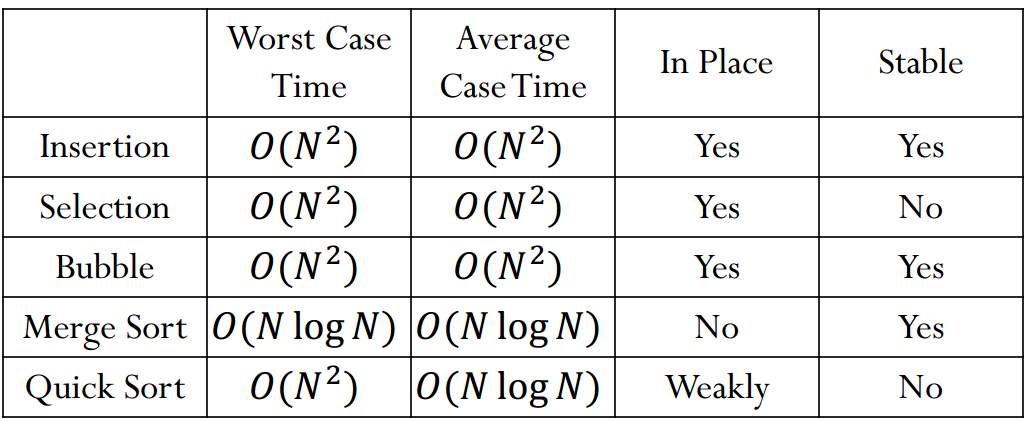
\includegraphics[scale=0.4]{P1.png}
\end{figure}
\par However, we need to test the algorithms' time efficiency by ourselves, so I wrote a cpp file to print out the time required for each algorithm, which is included in appendix part.
\section{Result}
To test time efficiency, I used clock() function to get the time required. To get rid of other disturbing factor, I used to variable start and stop to get the time right before and after the sorting complete, then their difference is the time used. In my analysis, I get 10 set of data ,from which the sorted array' size is 1, 10, 50, 100, 500, 1000, 5000, 25000 and 100000.
\begin{table}[H]
\centering
\begin{tabular}{|c|c|c|c|c|c|c|c|c|c|}
\hline
Data Size                 & 1    & 10   & 50     & 100    & 500    & 1000   & 5000   & 25000  & 100000 \\ \hline
Bubble Sort               & 3e-6 & 4e-6 & 2.7e-5 & 1.1e-4 & 1.7e-3 & 0.0057 & 0.053  & 1.4    & 24     \\ \hline
Insertion Sort            & 1e-6 & 3e-6 & 1.4e-5 & 5.4e-5 & 8.1e-4 & 0.0011 & 0.018  & 0.45   & 7.2    \\ \hline
Selection Sort            & 1e-6 & 3e-6 & 1.7e-5 & 6.3e-5 & 9e-4   & 0.0011 & 0.019  & 0.46   & 7.2    \\ \hline
Merge Sort                & 1e-6 & 5e-6 & 1.8e-5 & 4.8e-5 & 2e-4   & 1.4e-4 & 5.6e-4 & 0.0033 & 0.015  \\ \hline
Quick Sort (not in-place) & 1e-6 & 4e-6 & 1.9e-5 & 4.3e-5 & 2.1e-4 & 1.6e-4 & 6.5e-4 & 0.0036 & 0.016  \\ \hline
Quick Sort (in place)     & 1e-6 & 4e-6 & 1.7e-5 & 3.7e-5 & 2e-4   & 1.4e-4 & 5.6e-4 & 0.0032 & 0.014  \\ \hline
\end{tabular}
\end{table}
\begin{figure}[H]
\centering
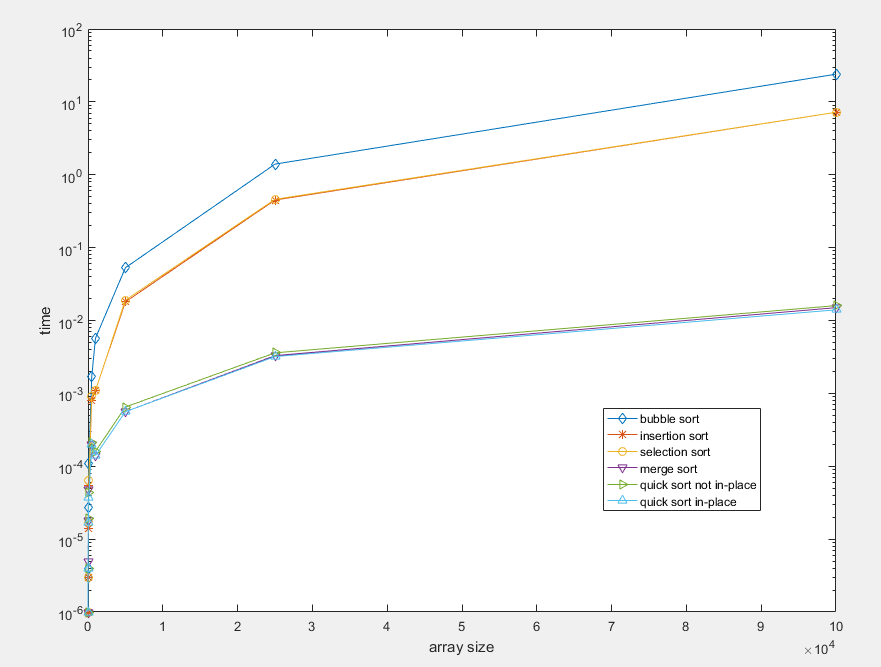
\includegraphics[scale=0.55]{P2.png}
\end{figure}
\section{Conclusion}
This chart is plot by matlab, showing the time efficiency of each algorithms compared to each other, and it has following characteristics.
\begin{enumerate}
\item The average time required for each algorithm grows as the array grows bigger.
\item As shown in the graph before, bubble sort, insertion sort and selection sort require much more time to sort huge array than the other sort algorithms. However, when the data size is extremely small, there is no such characteristic and the insertion sort and selection sort even requires less time than merge sort and quick sort.
\item Even though insertion sort, selection sort and bubble sort have the same time complexity as shown in the graph from lecture, it seems that bubble sort needs more time to sort than others. I guess its because bubble sort needs to compare every two members of the array once.
\end{enumerate}
\section{Appendix}
The appendix shows the cpp code for time comparison.
\begin{figure}[H]
\centering
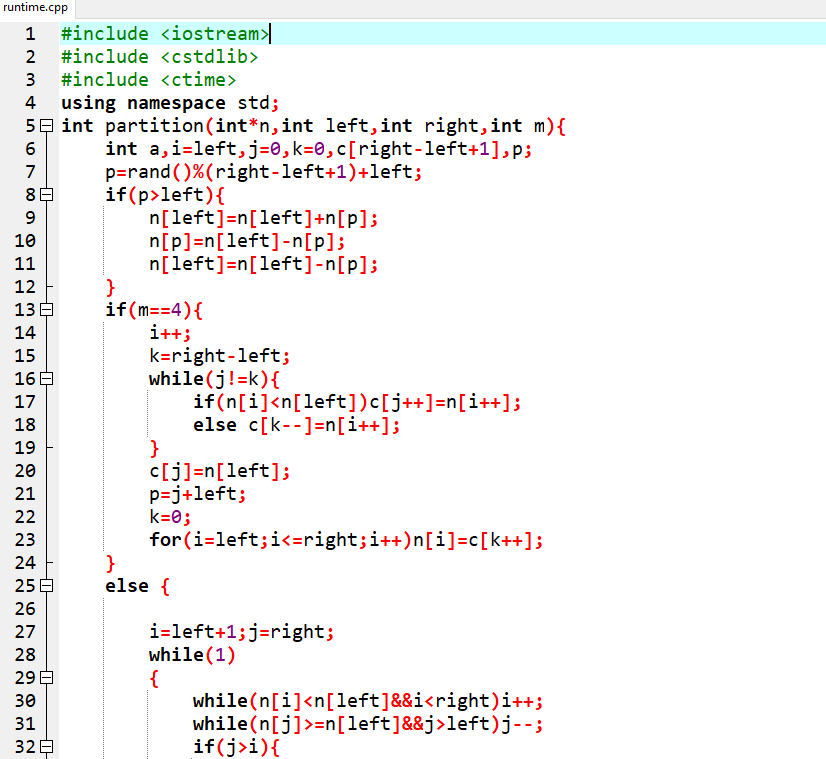
\includegraphics[scale=0.6]{P3.png}
\end{figure}
\begin{figure}[H]
\centering
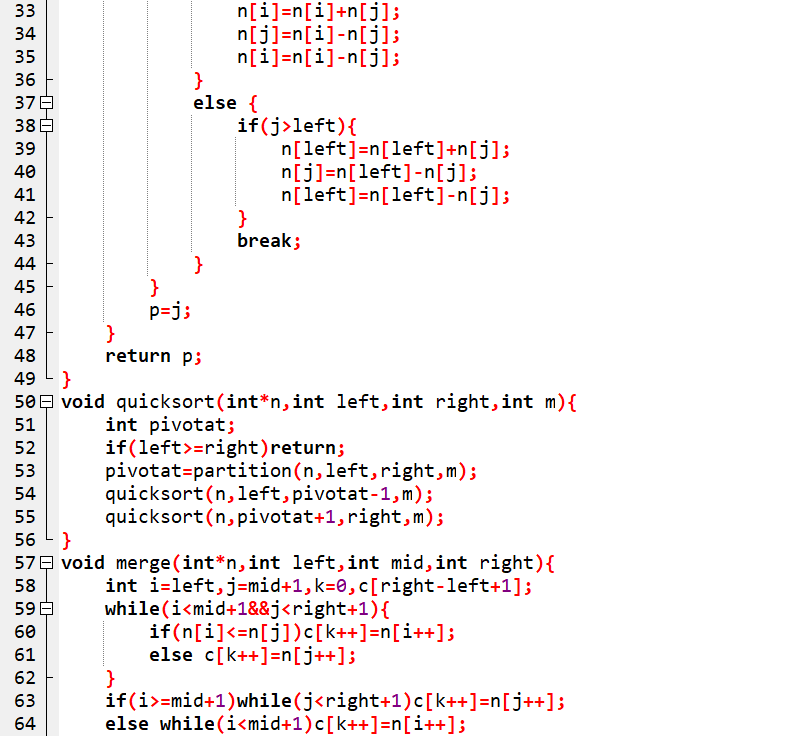
\includegraphics[scale=0.6]{P4.png}
\end{figure}
\begin{figure}[H]
\centering
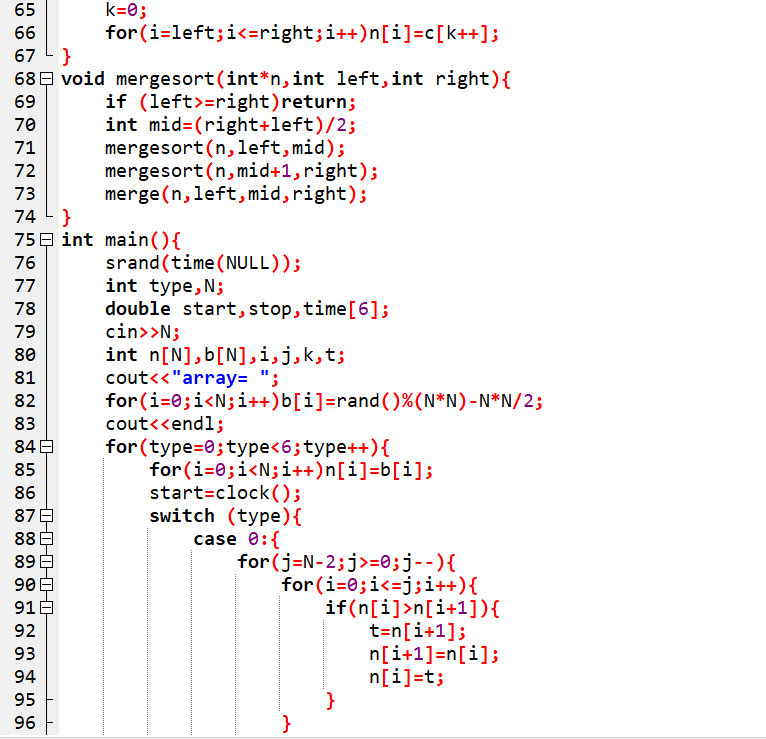
\includegraphics[scale=0.6]{P5.png}
\end{figure}
\begin{figure}[H]
\centering
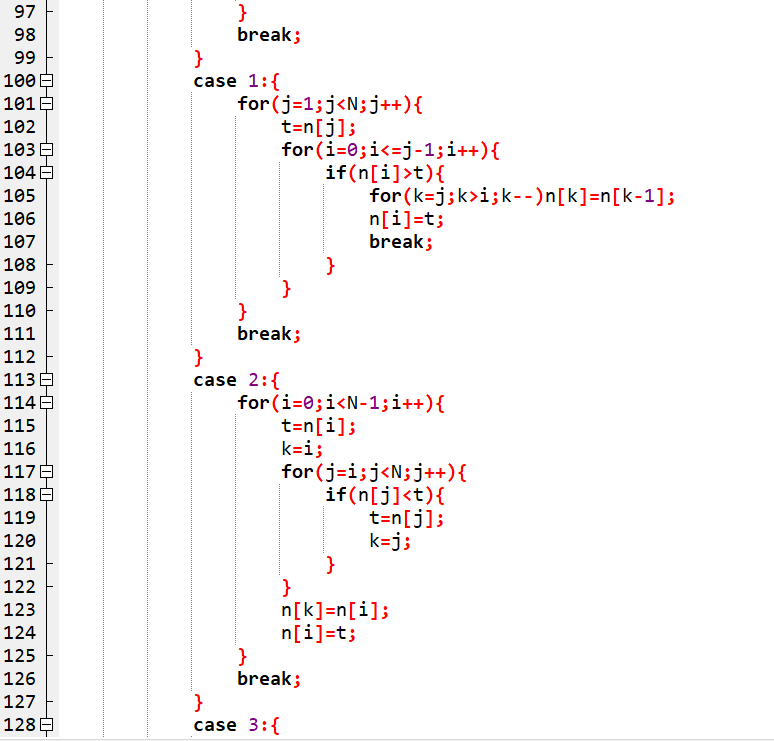
\includegraphics[scale=0.6]{P6.png}
\end{figure}
\begin{figure}[H]
\centering
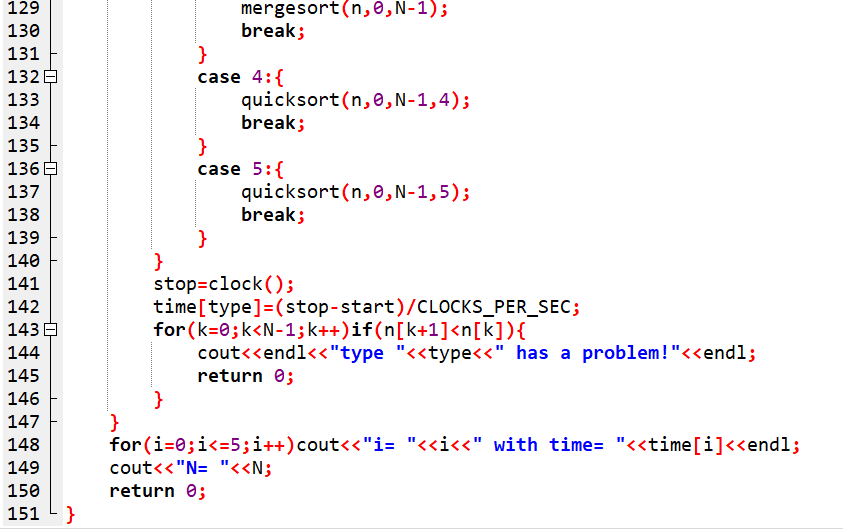
\includegraphics[scale=0.6]{P7.png}
\end{figure}
Then the appendix shows the cpp code for each sort algorithm
\begin{figure}[H]
\centering
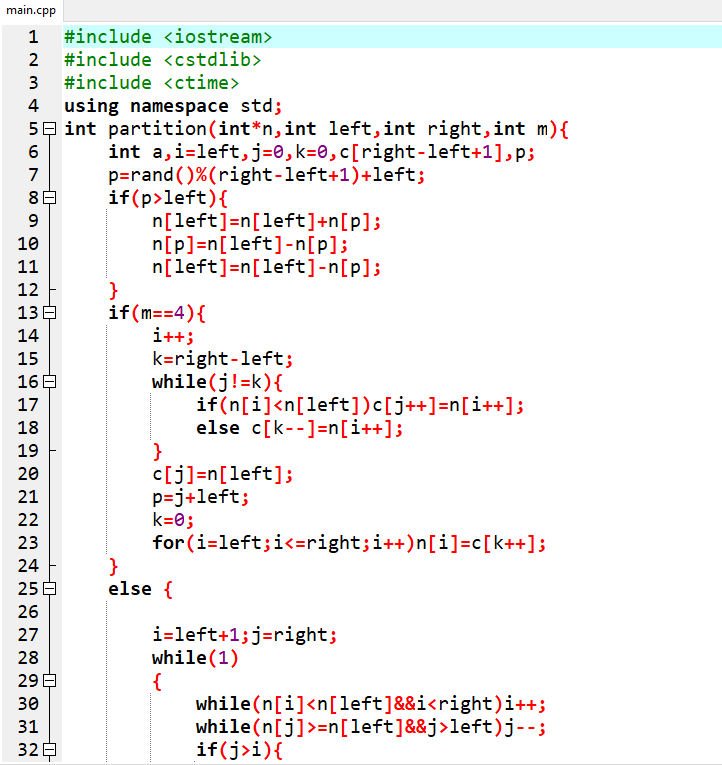
\includegraphics[scale=0.6]{P8.png}
\end{figure}
\begin{figure}[H]
\centering
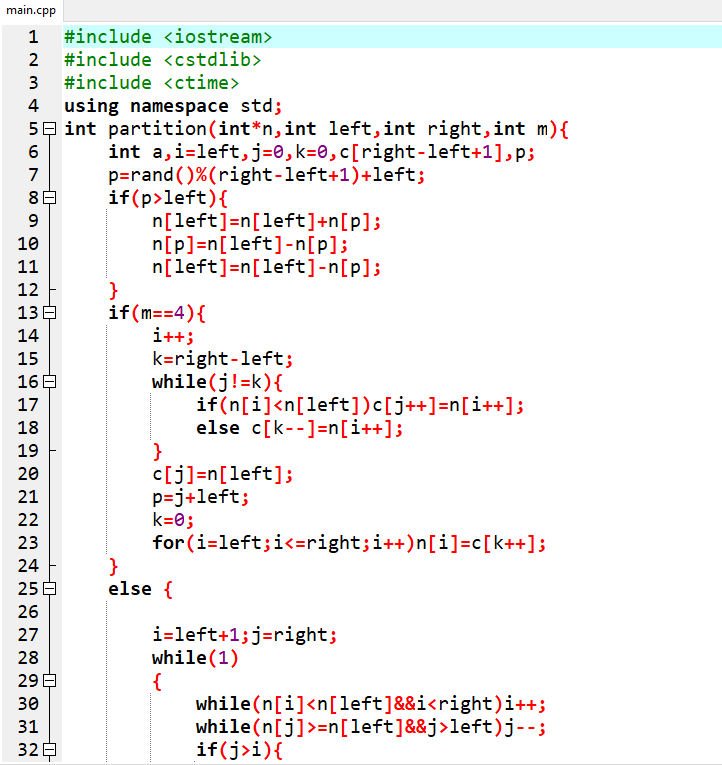
\includegraphics[scale=0.6]{P8.png}
\end{figure}
\begin{figure}[H]
\centering
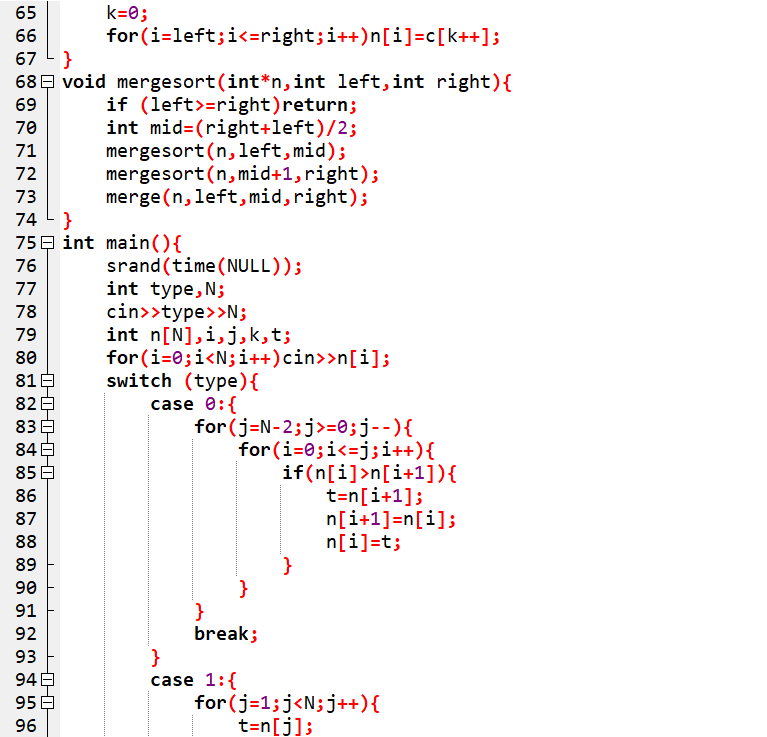
\includegraphics[scale=0.6]{P10.png}
\end{figure}
\begin{figure}[H]
\centering
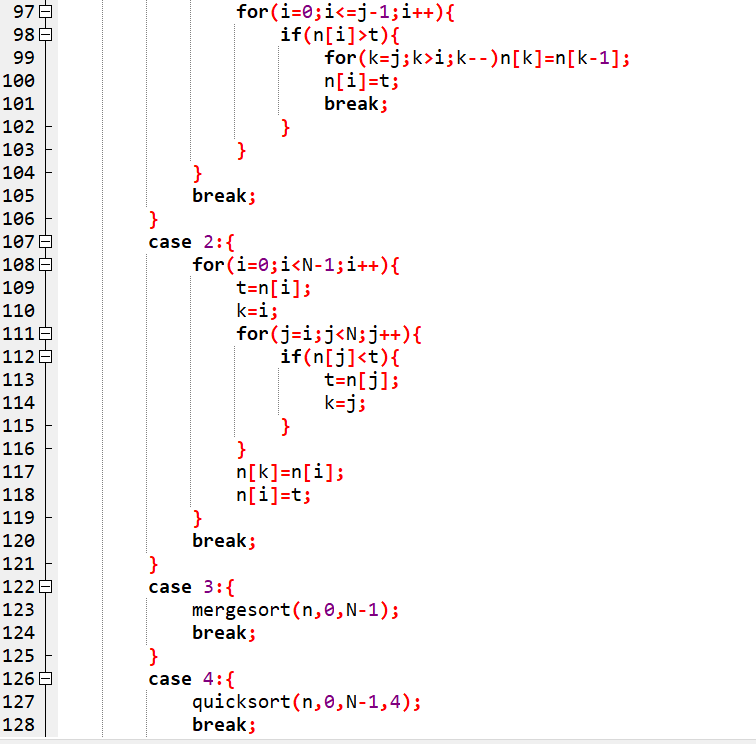
\includegraphics[scale=0.6]{P11.png}
\end{figure}
\begin{figure}[H]
\centering
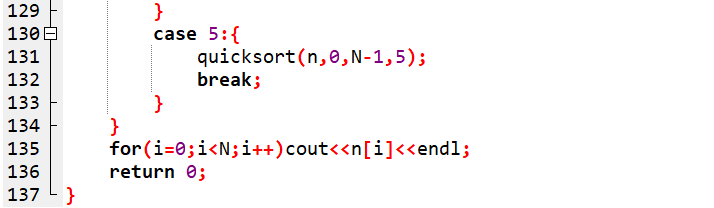
\includegraphics[scale=0.6]{P12.png}
\end{figure}
\end{document}